\chapter{Evaluation}
\label{ch:evaluation}
This chapter explains how the implementations were tested together with the results.
The first section explains how the Lucene and the Elasticsearch experiments were conducted.
Section \ref{sec:results} shows the results and how the results were obtained,
and section \ref{sec:discussion} discusses the results.
Lastly, section \ref{sec:reasearch-questions-evaluation} evaluates the research questions agains the results.

\section{Experimental Setup}
- Why are there two experiments.
- Author discovered Elasticsearch's plugin API after implementing query expansion in lucene after looking into how to move the implementation into Elasticsearch.
- Elasticsearch plugin API have very limited documentation.
- Hard to implement.
- Create an illustration on what is measured. Client -> web server -> search engine. Different measurementes

\subsection{Lucene Experiment}
The Lucene experiments starts to build the index with all the photo data.
To make the experiment simpler only the fields: tags, title and url are stored.

\subsection{Elasticsearch Experiment}
The Elasticsearch experimental setup contains two main components, a web server and a search engine.
The web server is implemented in NodeJS and the search engine used is Elasticsearch.

As large applications ofter use cloud providers, the tests also needed to be conducted using cloud providers.
The requirement set for the cloud provider was: need to be videly used, have servers in Europe and provide VPS services.
Possible providers were: Amozon Web Services\footnote{\url{https://aws.amazon.com/}},
Google Cloud Platform\footnote{\url{https://cloud.google.com/}} and Digital Ocean\footnote{\url{https://www.digitalocean.com/}}.
Google Cloud Platform were chosen as the service provider, as you have more flexibility to choose between number of cores and the memory size,
the author had both knowledge to the platform and they gave away free credits[?? Maybe give a better reason?].
Tests were conducted using two Google Compute Engine instances.
Web services always strives to place the servers as close to the users as possible.
To make the experiment simulate a real world scenario both the instances were placed in the reagion called \textit{europe-west1-c}.

\subsubsection{Elasticsearch Instance}
The instance running Elasticsearch had the following specifications: 2 vCPUs, 10 GB memory and 20 GB SSD.
Elasticsearch's documentation\footnote{\url{https://www.elastic.co/guide/en/elasticsearch/guide/current/hardware.html}}
suggest that memory will be the most important resource in most use cases.
As a result more memory were chosen over the number of CPUs.
An important setting in Elasticsearch is the heap size.
By default the heap memory size is set to 1 GB, but were changed to 5 GB in the test environment.
A logical asumption would be to set the Elasticsearch to use all the available memory, except the memory needed for the operating system.
However, Elasticsearch's underlying structure Lucene also needs memory.
Lucene stores the data in separate files.
The datastructure inside the files are immutable, which makes them optimized for caching.
With this strategy Lucene optimizes the underlying operating system's eager to hold small and often used files in memory.
According to the Elasticsearch documentation\footnote{\url{https://www.elastic.co/guide/en/elasticsearch/guide/current/heap-sizing.html}}
the heap size should be set to 50\% or less, of the available memory.

Most operating systems today also comes with swapping turned on by default.
If the operating system decides to swap it would significantly reduce the performance.
To avoid the problem swapping were turned off on the Elasticsearch instance.

\subsubsection{NodeJS Instance}
The instance running NodeJS had the following specifications: 4 vCPUs, 4 GB memory and 10 GB SSD.
On the web server we want to be able to handle as many requests as possible.
The number of requests the server is able to handle are closely linked to the number of cores.
That is why the Node.js instance has more cores at the cost of less memory.

Node.js is by design single threaded, which would make 3 of the cores on the Node.js server being idle.
However, this problem can be solved by using tool called pm2\footnote{\url{http://pm2.keymetrics.io/}}.
pm2 has a feature called \textit{cluster mode}, which may spawn multple Node.js instances.
To allow maximum CPU utilization, pm2 can be configured to spawn as many Node.js instances as the number of cores.

To test the implementation the Node.js web server implemented two different endpoints.

- Node.js, version
- Configuration NODE\_ENV=production
- pm2
- two endpoints, one for base line one for query expansion

\subsection{Data Set}
\label{sec:dataset}
The data set consits of photo data gathered from the Flickr API\footnote{\url{https://www.flickr.com/services/api/}}.
The data set is gathered over

All the data are gathered over the periode january to may.
The data set used in the experiment consists of 4,561,816 photos and 9,993,411 tags.
Of all the photos, a total of 1,708,324 photos have 1 or more tags.
Which means that 37 \% of the photos have tags.

Analysing the data set discovered that each photo have an average of [??] tags.
A total of [??] images have no tags and [??] have atleast 1 tag.

\begin{figure}[h!]
  \centering 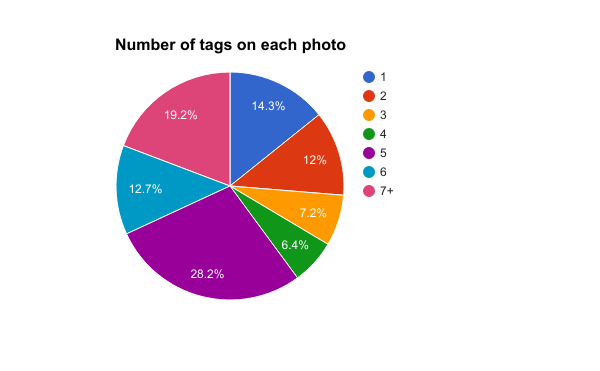
\includegraphics[width=1\linewidth]{img/number-of-tags-distribution.png}
  \caption{Pie chart that shows the distribution on how many tags each photo have.}
  \label{fig:result-vary-result-size}
\end{figure}

\subsection{Performance Metrics}
Evaluating the implementation is done by measuring the response time from a client sends the request to the response arrives.


\begin{figure}[h!]
  \centering 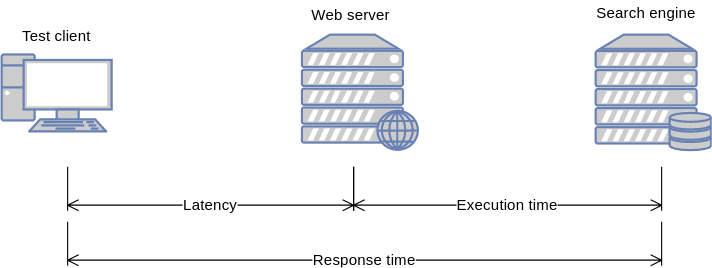
\includegraphics[width=0.9\linewidth]{img/latency-measurements.png}
  \caption{Overview of the different measurements used when evaluating the implementation.}
  \label{fig:latency-measurements}
\end{figure}

\section{Results}
\label{sec:results}
The results from the experiments in the project report [??],
showed that the query expansion implementation had about 2 times longer latency compared to the baseline implementation.
The latency were measured from the request left the user to the response from the server arrived.

All the results show that the first request is often the slowest.
After the initial request the respons is cached by Lucene and makes all the subsequent requests a lot faster.

\subsection{Lucene Results}
About 50\% increased latency with the Lucene implementation.
Can see that Lucene heavily caches search result.
The first initial results often is a lot slower than the subsequent searces.

\subsection{Elasticsearch Experiment Results}
To evaluate the performance of the plugin developed a few tests were conducted.
All of the tests were done in two different ways,
one prewaring the cache and one without prewaring the cache.


\begin{figure}[h!]
  \centering 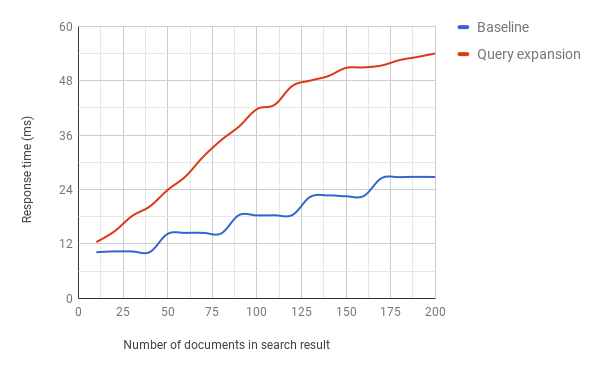
\includegraphics[width=1\linewidth]{img/result-vary-result-size.png}
  \caption{Overview of the different measurements used when evaluating the implementation.}
  \label{fig:result-vary-result-size}
\end{figure}

\begin{figure}[h!]
  \centering 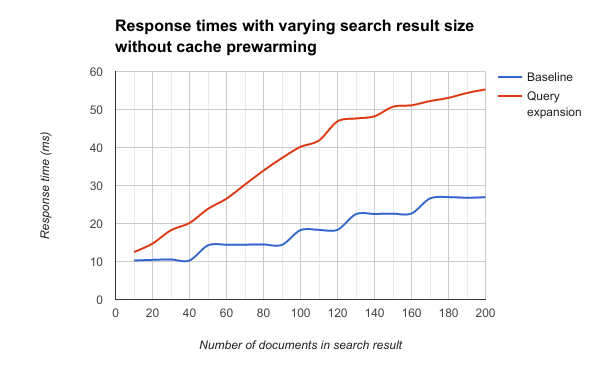
\includegraphics[width=1\linewidth]{img/result-vary-result-size-without-cache.png}
  \caption{Overview of the different measurements used when evaluating the implementation.}
  \label{fig:result-vary-result-size}
\end{figure}

\section{Discussion}
\label{sec:discussion}
On Elastic's offical website there is a discussion about devoloping plugins for Elasticsearch.
The quote below is an answer from the Elastic developer Adrien Grand on wheter there exists an offical guide on how to develop Elasticsearch plugins \cite{elasticsearch-plugin-quote}.

\begin{quote}
  No, there is no guide about writing plugins and the API is actually quite unstable.
  The plugin API is mainly a way for us to provide additional functionality through plugins so that we do not have to fold everything into a single release artifact that would be quite huge.
  Some community membors have writter plugins by taking inspiration of existing plugins but we do not want to commit on a stable API for plugins as this might prevent us from improving other areas of elasticsearch.
\end{quote}

\section{Research Question Evaluation}
\label{sec:reasearch-questions-evaluation}
\begin{enumerate}
  %\item How to provide instant personalized recommendations on a cold start based on the query typed?
  \item \textbf{How to achieve more relevant search results based on a query from a user?} \newline
  As mentioned in section \ref{sec:problem-specification} the main focus areas were scaling and latency.
  Therefore, the relevance was never measured.
  Based on the work by Rudihagen,
  this project report assumes that query expansion returns more relevant results compared to the baseline search.

  \item\label{rq:scaling} \textbf{How to make the search recommandation scale with an increasing amount of data?} \newline
  As mentioned earlier, Elasticsearch is proven to scale to petabytes of data \cite{elasticsearch-scale},
  if configured correctly, and was thus used as the search engine for this project report.
  Rudihagen's implementation also used Elasticsearch, and was configured with one index for each user.
  This configuration is fine for most cases, but according to the documentation this does not scale well if you have a large user base \cite{elasticsearch-indices}.

  Elasticsearch require proper tuning and configuration.
  Without testing the solution on a large data we cannot conclude that the implementation would scale,
  but the current implementation have potential to scale.

  \item\label{rq:latency} \textbf{How to develop a search recommendation method that fulfills the interactive requirements?} \newline
  From the results we can see that the implementation are delivering results in about 16 ms, in a test environment.
  However, the query expansion implementation has a latency which is about 2 times greater than the baseline.
  For real world use cases, this might exceed the latency to above the interactivity limit.
\end{enumerate}

\section{Notes}
- During testing the same query sometimes gave different results. Because of this: https://www.elastic.co/blog/understanding-query-then-fetch-vs-dfs-query-then-fetch
- Show example results. Same query, but one with query expansion and one without.
